% =====================================================================
\chapter{Các thành phần hệ thống}\label{chap:thanhphan}
% =====================================================================

Chương này liệt kê mọi thành phần phần cứng và phần mềm của hệ thống, kèm các thông
số quan trọng quyết định thiết kế. Lý do chọn từng thành phần được trình bày trong
các hộp \emph{Lý do}; phần kiến trúc tổng thể nằm ở Chương~\ref{chap:thietke}.

\section{Tổng quan ba nút phần cứng}
\begin{table}[H]
\centering\small
\caption{Ba nút phần cứng và vai trò}\label{tab:nodes}
\begin{tabularx}{\linewidth}{@{}lXl@{}}
\toprule
\textbf{Nút} & \textbf{Thiết bị gắn kèm và nhiệm vụ} & \textbf{Mã nguồn} \\ \midrule
Máy chủ (ESP32-C3) & TFT ST7789, 2 servo SG90, còi. Nhận UDP, quản lý phiên RFID, tính phí, điều khiển thanh chắn, web server, mDNS & \file{Server/main/} \\
Sensor Client (ESP8266) & 5 cảm biến IR, cảm biến lửa, cảm biến mực nước. Lọc nhiễu và gửi trạng thái & \file{SensorClient/} \\
RFID Client (ESP8266) & 2 đầu đọc MFRC522, DHT11. Phát Wi-Fi, gửi sự kiện quẹt thẻ & \file{RFIDClient/} \\
\bottomrule
\end{tabularx}
\end{table}

\section{Vi điều khiển}
\subsection{ESP32-C3 SuperMini (máy chủ)}
\begin{table}[H]
\centering\small
\caption{Thông số quan trọng của ESP32-C3 SuperMini}\label{tab:esp32c3}
\begin{tabularx}{\linewidth}{@{}lX@{}}
\toprule
CPU & RISC-V 32 bit, 1 nhân, chạy ở 160\,MHz \\
Bộ nhớ & 400\,KB SRAM (ứng dụng dùng được $\approx$ 321\,KB DRAM), 384\,KB ROM \\
Flash & Flash ngoài, cấu hình 2\,MB; phân vùng ứng dụng 1,5\,MB \\
Không dây & Wi-Fi 802.11 b/g/n 2,4\,GHz, Bluetooth LE 5 \\
Ngoại vi dùng tới & SPI2 có GDMA, LEDC (PWM 14 bit), GPIO, bộ định thời \code{esp\_timer} 64 bit \\
Nạp/gỡ lỗi & USB Serial/JTAG tích hợp (không cần chip USB-UART, không cần driver) \\
Kích thước & $22\times18$\,mm \\
\bottomrule
\end{tabularx}
\end{table}

\begin{table}[H]
\centering\small
\caption{So sánh phương án vi điều khiển cho máy chủ}\label{tab:mcu}
\begin{tabularx}{\linewidth}{@{}lXXXX@{}}
\toprule
\textbf{Tiêu chí} & \textbf{ESP32-C3} & \textbf{ESP32} & \textbf{ESP8266} & \textbf{Arduino Uno} \\ \midrule
CPU & RISC-V 160\,MHz & Xtensa 2 nhân 240\,MHz & Xtensa 80/160\,MHz & AVR 16\,MHz \\
SRAM & 400\,KB & 520\,KB & $\sim$80\,KB & 2\,KB \\
Wi-Fi & Có & Có & Có & Không \\
PWM phần cứng & LEDC 14 bit & LEDC & PWM mềm & 8 bit \\
SPI có DMA & Có & Có & Hạn chế & Không \\
RTOS chính thức & FreeRTOS & FreeRTOS & Hạn chế & Không \\
\bottomrule
\end{tabularx}
\end{table}

\begin{lydo}
Máy chủ phải \emph{đồng thời} giữ Wi-Fi, chạy web server và UDP server, vẽ màn hình
$240\times240$ màu 16 bit và phát PWM cho servo. Chỉ riêng ảnh màn hình đã cần
$240\times240\times2 = 115\,200$ byte RAM — lớn hơn toàn bộ RAM của ESP8266 hay
Arduino. ESP32-C3 có đủ RAM, có DMA cho SPI (CPU không phải chờ khi đẩy ảnh), có PWM
phần cứng (servo không rung khi CPU bận mạng) và được hỗ trợ chính thức bởi
ESP-IDF/FreeRTOS. So với ESP32 bản gốc, C3 rẻ và nhỏ hơn; một nhân 160\,MHz đã dư
năng lực cho bài toán này.
\end{lydo}

\subsection{ESP8266 NodeMCU (hai client)}
\begin{table}[H]
\centering\small
\caption{Thông số quan trọng của ESP8266}\label{tab:esp8266}
\begin{tabularx}{\linewidth}{@{}lX@{}}
\toprule
CPU & Tensilica L106 32 bit, 80\,MHz \\
Bộ nhớ & $\sim$80\,KB RAM dữ liệu cho người dùng, flash 4\,MB trên bo NodeMCU \\
Ngoại vi dùng tới & 1 kênh ADC 10 bit (A0), SPI phần cứng (HSPI), GPIO \\
Không dây & Wi-Fi 802.11 b/g/n, chạy được chế độ STA hoặc AP \\
\bottomrule
\end{tabularx}
\end{table}

\begin{lydo}
Nút cảm biến chỉ đọc vài chân số, một chân ADC, giao tiếp SPI với RC522 và gửi gói
UDP nhỏ — nhu cầu tính toán rất thấp. ESP8266 là bo Wi-Fi rẻ và phổ biến nhất, có
ADC, có hệ sinh thái thư viện Arduino lớn (MFRC522, DHT, ArduinoOTA). Tách ra hai
bo vì máy chủ không đủ chân: màn hình, servo và còi đã dùng 9 chân trong khoảng 13
chân khả dụng của ESP32-C3 SuperMini.
\end{lydo}

\section{Thiết bị chấp hành và hiển thị}
\begin{table}[H]
\centering\small
\caption{Thiết bị chấp hành, hiển thị và thông số quan trọng}\label{tab:actuators}
\begin{tabularx}{\linewidth}{@{}p{3.1cm}X@{}}
\toprule
\textbf{Thiết bị} & \textbf{Thông số quan trọng} \\ \midrule
TFT ST7789 1,54" & $240\times240$, IPS, 262K màu (dùng RGB565 16 bit), SPI chỉ ghi, chu kỳ ghi tối thiểu $\approx$ 16\,ns ($\approx$ 62\,MHz); hệ thống chạy 40\,MHz \\
Servo SG90 $\times2$ & 4,8–6\,V; mô-men $\approx$ 1,8\,kg$\cdot$cm; tốc độ $\approx$ 0,1\,s/60°; điều khiển PWM 50\,Hz, xung $\approx$ 500–2400\,µs cho 0–180° \\
Còi (module) & Tích cực mức thấp: chân tín hiệu mức 0 thì kêu \\
\bottomrule
\end{tabularx}
\end{table}

\section{Cảm biến}
\begin{table}[H]
\centering\small
\caption{Cảm biến, thông số và lý do lựa chọn}\label{tab:sensors}
\begin{tabularx}{\linewidth}{@{}p{2.9cm}p{4.0cm}X@{}}
\toprule
\textbf{Cảm biến} & \textbf{Thông số} & \textbf{Lý do lựa chọn} \\ \midrule
IR phản xạ HW-201 (họ FC-51) $\times5$ & 2–30\,cm, so sánh LM393 có biến trở, ngõ ra số tích cực mức thấp & Rẻ, phát hiện vật ở cự ly vài cm hợp với xe mô hình, chỉ tốn 1 chân. Siêu âm chính xác hơn nhưng tốn 2 chân/cảm biến và phải đo thời gian. \\
Cảm biến lửa (module 4 chân AO/DO) & Bước sóng 760–1100\,nm, góc $\approx$ 60°, ngõ ra số có ngưỡng & Phản ứng nhanh hơn cảm biến khói/nhiệt; ngõ ra số sẵn ngưỡng. \\
Mực nước (điện trở) & Vùng đo $\approx$ 40\,mm, ngõ ra tương tự & Đơn giản, chỉ cần 1 chân ADC, hợp với mô hình tầng hầm. \\
RFID MFRC522 $\times2$ & 13,56\,MHz, ISO 14443A (MIFARE), SPI, 3,3\,V, đọc vài cm & Đọc được thẻ phổ biến (thẻ sinh viên, móc khóa), thư viện ổn định, giá rẻ. \\
DHT11 & 0–50\,°C ($\pm$2\,°C), 20–90\%RH, đọc tối đa 1 lần/giây & Đủ cho giám sát môi trường, chỉ cần 1 chân. \\
\bottomrule
\end{tabularx}
\end{table}

\section{Mô hình thực tế và bố trí phần cứng}\label{sec:mohinh}
Hình~\ref{fig:model} là mô hình nhóm đã chế tạo. Đế và vách làm bằng bìa formex
trắng (nhẹ, dễ cắt khoét lỗ cho cảm biến, cách điện); 5 ô đỗ được kẻ vạch dọc vách
sau, phía trước là sân quay đầu và hai làn ra/vào nằm hai bên hộp điều khiển ở giữa.

\begin{figure}[H]
\centering
\begin{subfigure}[t]{0.49\linewidth}\centering
  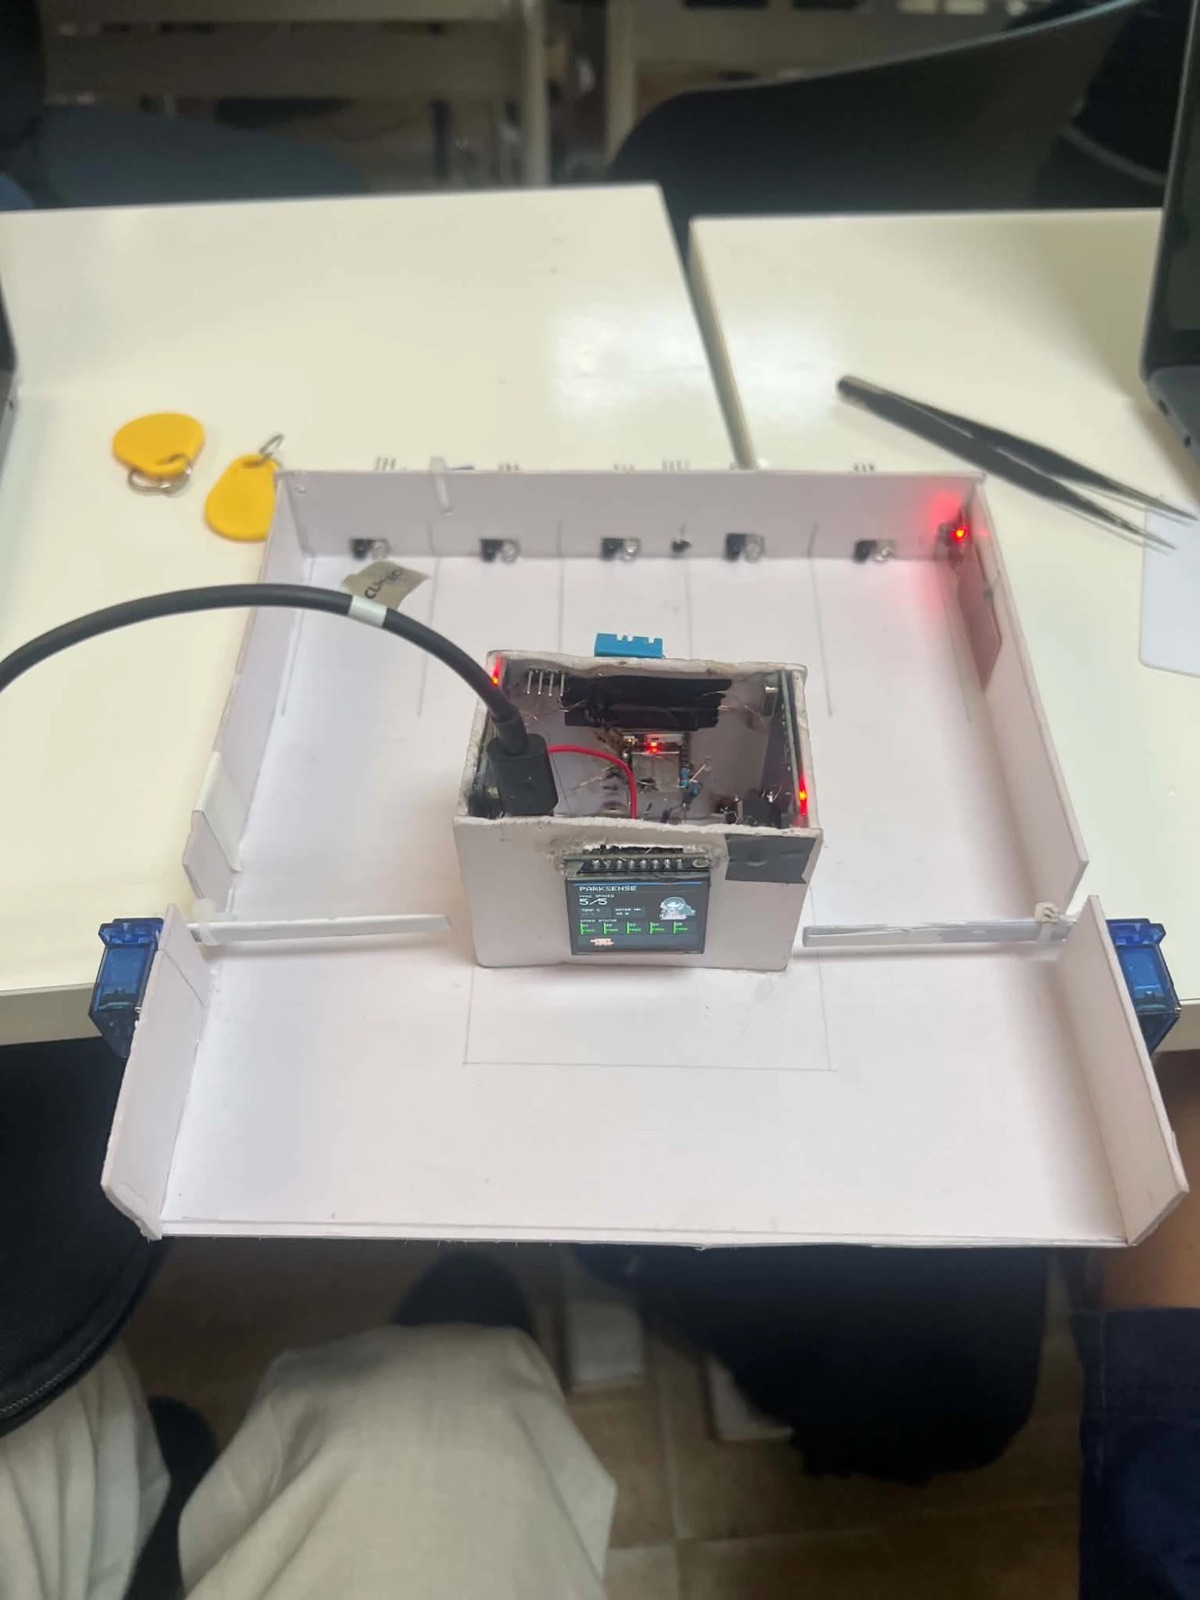
\includegraphics[width=\linewidth,height=0.36\textheight,keepaspectratio]{photos/model_top.jpg}
  \caption{Nhìn từ phía cổng: 5 ô đỗ, hộp điều khiển với TFT, hai thanh chắn servo}\label{fig:model-top}
\end{subfigure}\hfill
\begin{subfigure}[t]{0.49\linewidth}\centering
  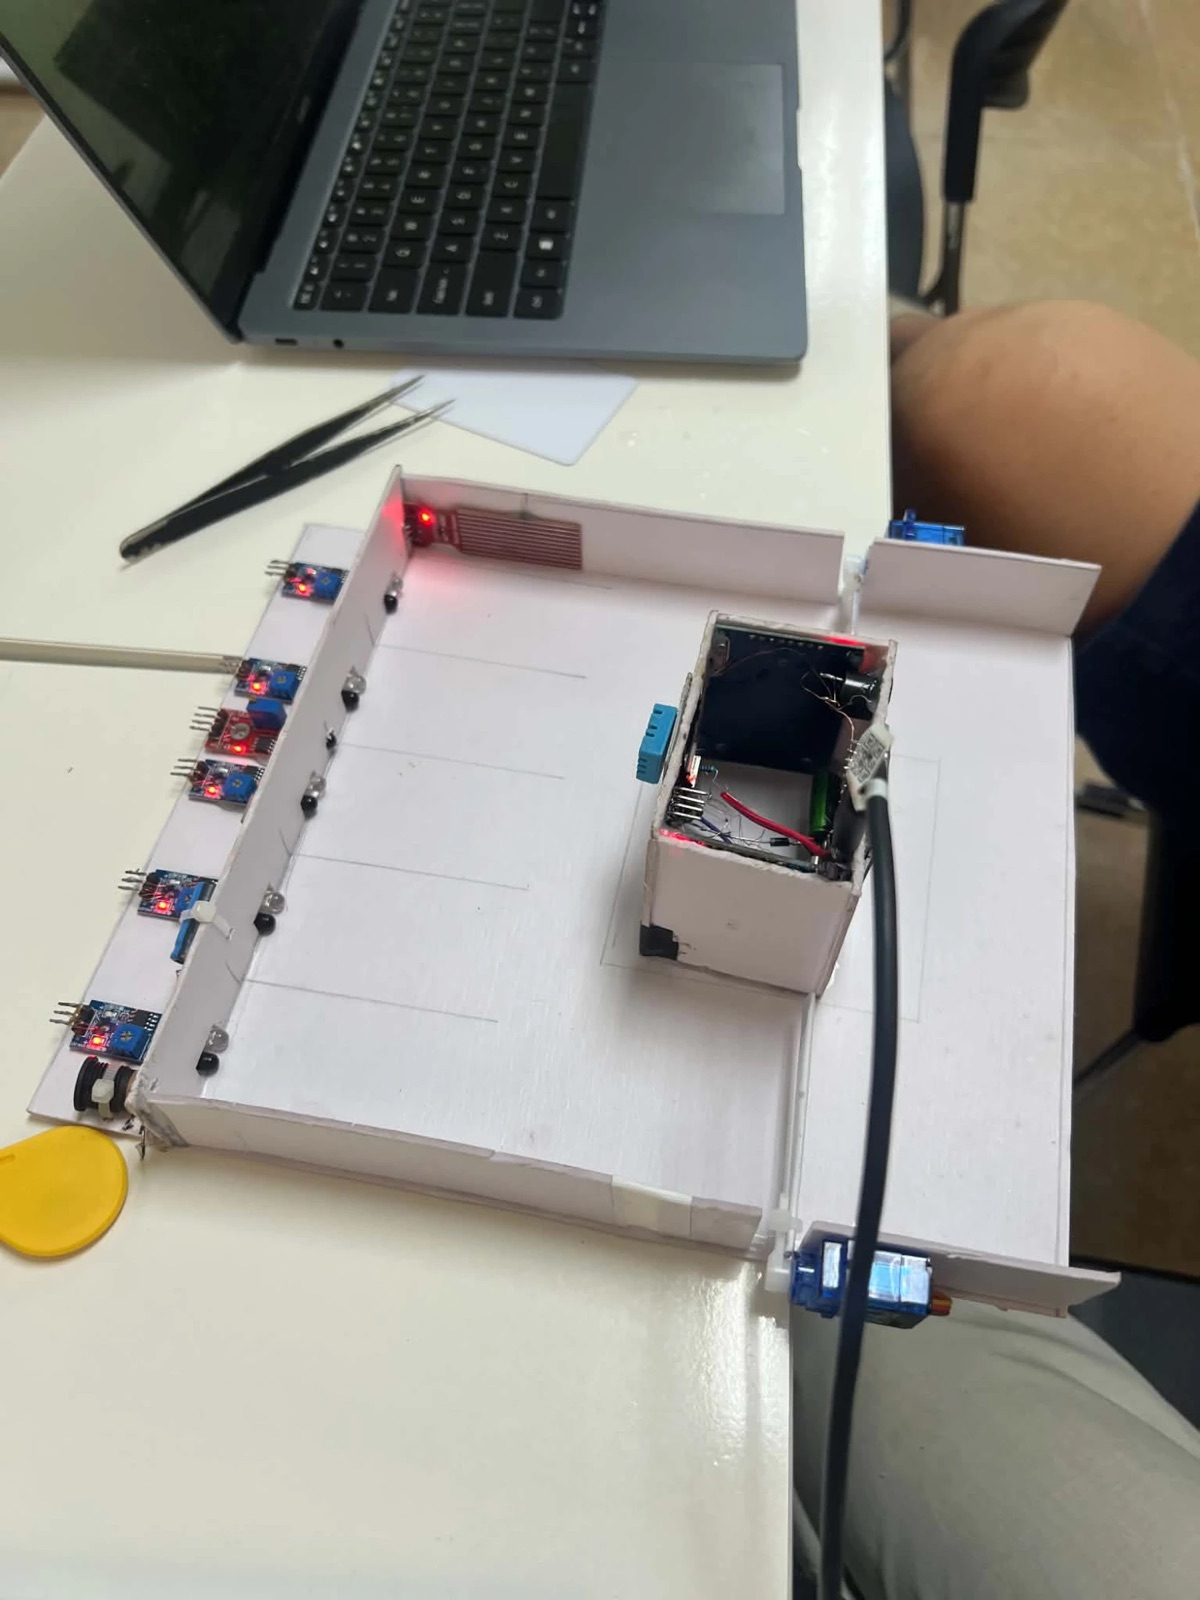
\includegraphics[width=\linewidth,height=0.36\textheight,keepaspectratio]{photos/model_angle.jpg}
  \caption{Góc nghiêng: dãy cảm biến ở mặt ngoài vách sau, cảm biến nước ở góc}\label{fig:model-angle}
\end{subfigure}

\vspace{4pt}
\begin{subfigure}[t]{0.49\linewidth}\centering
  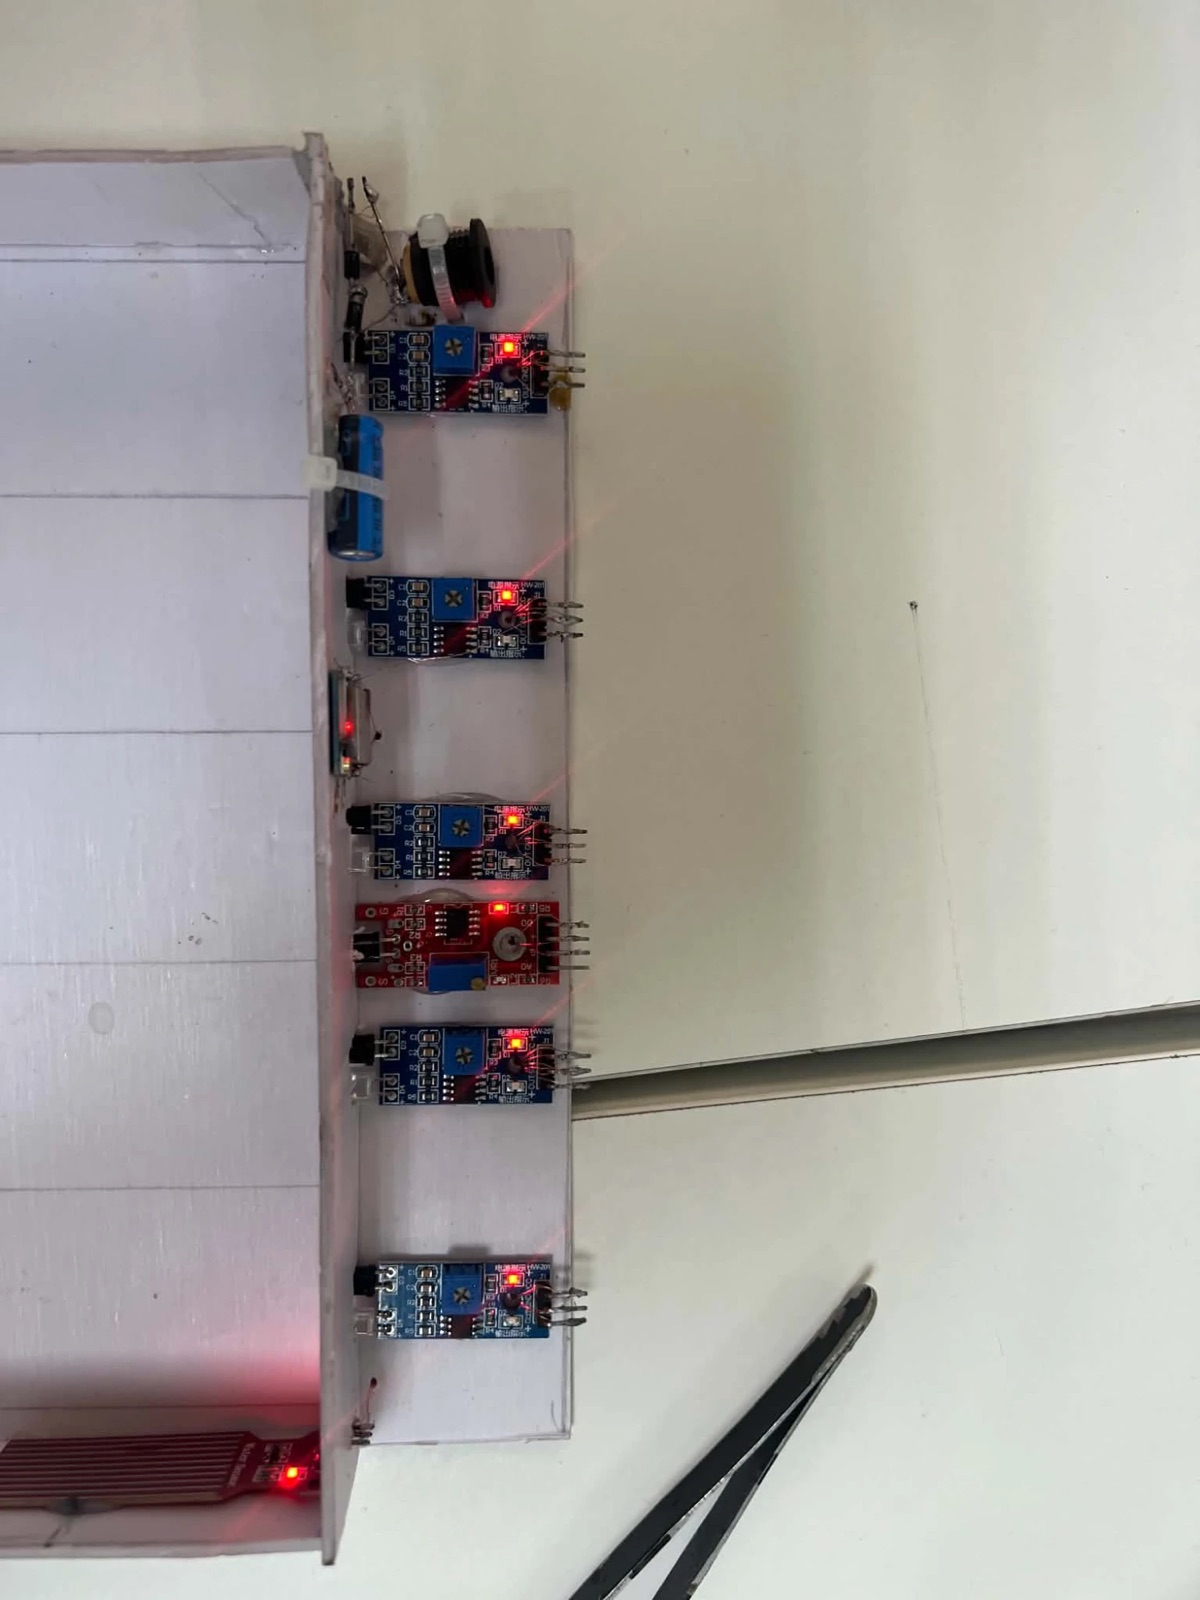
\includegraphics[width=\linewidth,height=0.36\textheight,keepaspectratio]{photos/model_sensorwall.jpg}
  \caption{Mặt ngoài vách sau: 5 module IR HW-201, module lửa (đỏ), jack nguồn DC, diode và tụ lọc}\label{fig:model-wall}
\end{subfigure}\hfill
\begin{subfigure}[t]{0.49\linewidth}\centering
  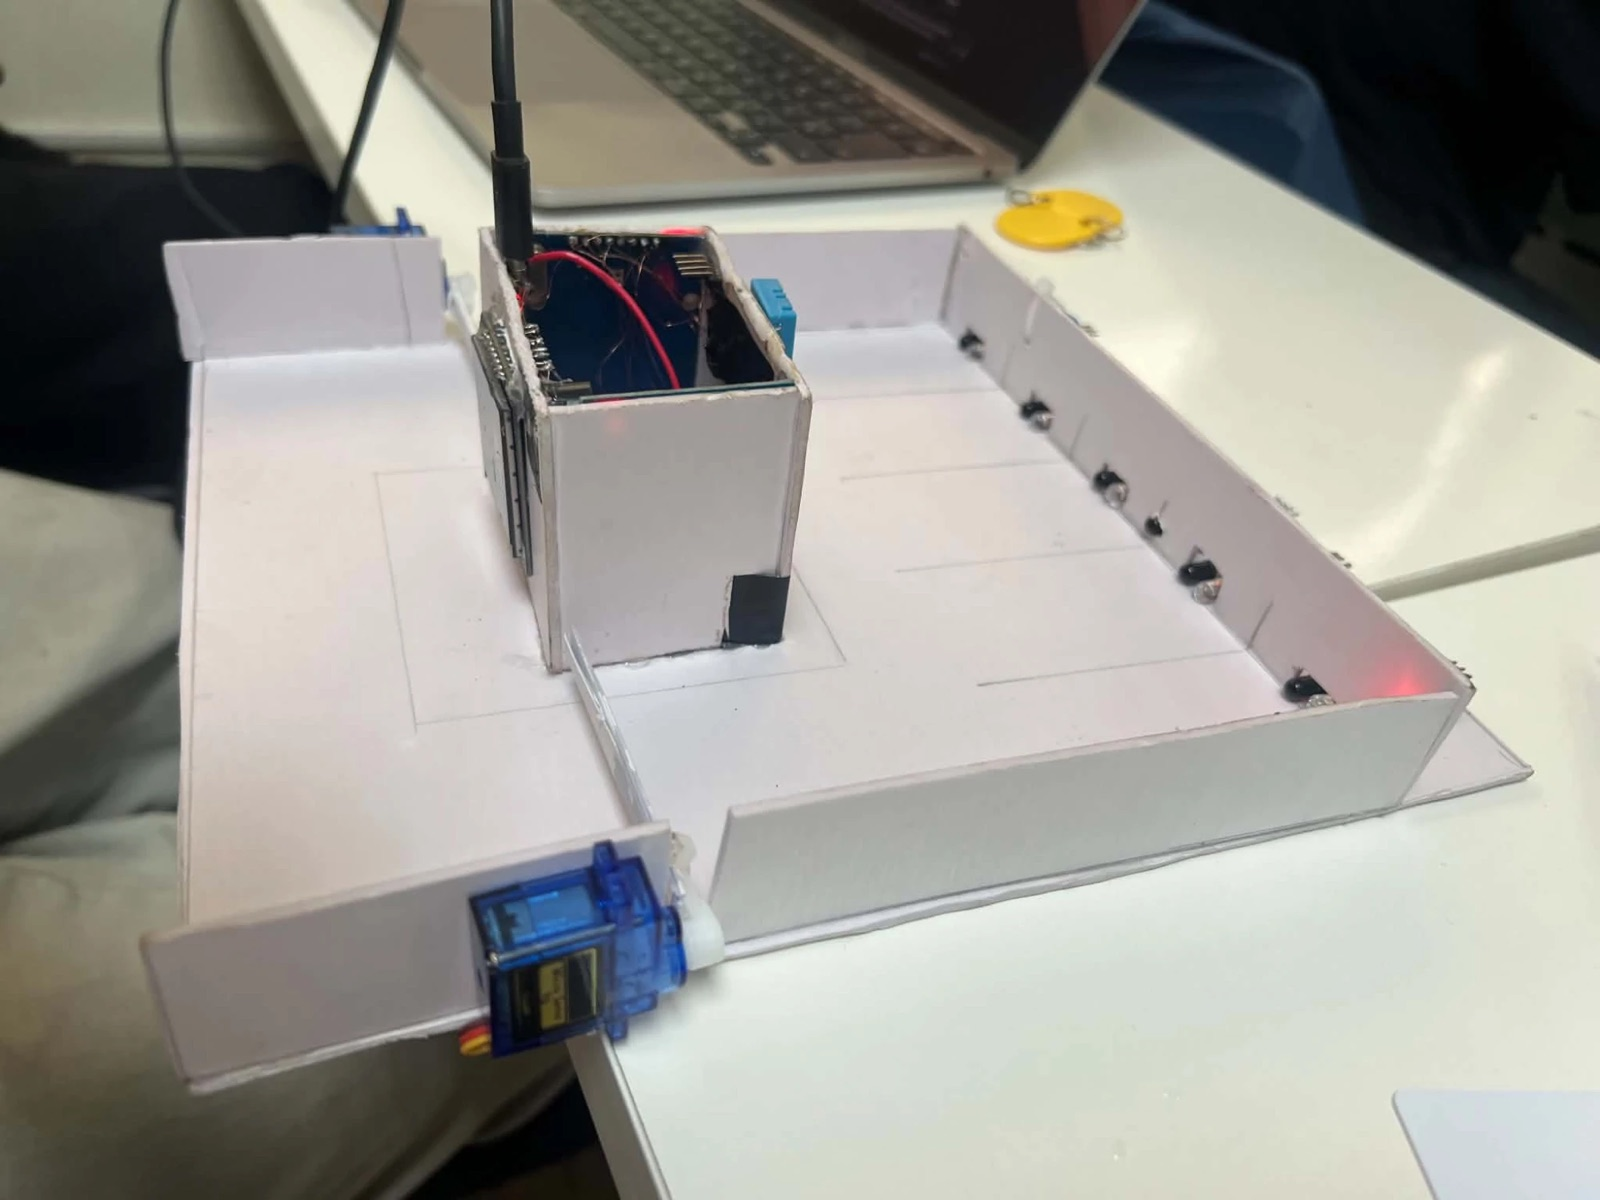
\includegraphics[width=\linewidth,height=0.36\textheight,keepaspectratio]{photos/model_gate.jpg}
  \caption{Cổng: servo SG90 gắn ở đầu vách, cần chắn quay ngang làn xe; DHT11 trên nóc hộp}\label{fig:model-gate}
\end{subfigure}
\caption{Mô hình bãi đỗ xe thông minh của nhóm}\label{fig:model}
\end{figure}

\begin{table}[H]
\centering\small
\caption{Vị trí lắp đặt từng thiết bị trên mô hình và lý do}\label{tab:placement}
\begin{tabularx}{\linewidth}{@{}p{3.1cm}p{4.3cm}X@{}}
\toprule
\textbf{Thiết bị} & \textbf{Vị trí} & \textbf{Lý do} \\ \midrule
5 module IR HW-201 & Mặt \emph{ngoài} vách sau, mỗi ô một module; LED phát/thu xuyên qua lỗ khoét vào đúng giữa ô & Dây và bo mạch nằm ngoài nên lòng bãi gọn, xe không vướng; khoảng cách tới đuôi xe chỉ vài cm, đúng tầm đo của IR. Mỗi module có biến trở chỉnh ngưỡng riêng theo độ phản xạ thực tế \\
Module lửa & Giữa dãy IR (giữa ô 3 và 4), đầu thu hướng vào lòng bãi & Góc nhìn $\approx$ 60° phủ được cả 5 ô từ vị trí trung tâm \\
Cảm biến mực nước & Góc trong của vách sau, sát sàn & Nước đọng tại điểm thấp và góc tường trước; đặt sát sàn để phát hiện sớm \\
Hộp điều khiển & Giữa bãi, giữa hai làn & Dây tới cảm biến, đầu đọc và servo đều ngắn; che bo mạch khỏi va chạm \\
TFT ST7789 & Mặt trước hộp, quay ra cổng & Người lái nhìn thấy số chỗ trống, hóa đơn và cảnh báo ngay khi tới cổng \\
2 đầu đọc RC522 & Hai hông hộp, mỗi đầu đọc quay ra một làn & Người lái quẹt thẻ từ trong xe ở đúng làn của mình; hai đầu đọc cách nhau cả hộp nên ít nhiễu chéo \\
2 servo SG90 & Đầu vách trái và phải, cần chắn quay ngang làn & Trục servo nằm ngoài làn, cần chắn nhẹ (nhựa) nên mô-men 1,8\,kg$\cdot$cm là dư \\
DHT11 & Nóc hộp điều khiển & Ra khỏi lòng hộp để không đo nhầm nhiệt do bo mạch tỏa ra \\
Jack DC, diode, tụ hóa & Mặt ngoài vách sau, cạnh dãy cảm biến & Một điểm cấp nguồn cho cả mô hình; xem đoạn ``Nguồn điện'' \\
\bottomrule
\end{tabularx}
\end{table}

\section{Sơ đồ chân}
\begin{table}[H]
\centering\small
\caption{Sơ đồ chân máy chủ ESP32-C3}\label{tab:pin-srv}
\begin{tabularx}{\linewidth}{@{}llX@{}}
\toprule
\textbf{Tín hiệu} & \textbf{GPIO} & \textbf{Ghi chú} \\ \midrule
TFT SCK / MOSI & 4 / 6 & SPI2 qua GPIO matrix; màn hình không cần MISO \\
TFT DC / RST / CS & 7 / 3 / 10 & Chọn lệnh–dữ liệu, reset, chọn chip \\
TFT đèn nền & 5 & Tắt khi khởi tạo để không thấy rác, bật sau khi sẵn sàng \\
Servo cổng vào / ra & 0 / 1 & Chân thường (bo không dùng thạch anh 32\,kHz) \\
Còi & 9 & Tích cực mức thấp; GPIO9 là chân strapping có kéo lên, trùng với trạng thái ``im lặng'' \\
\bottomrule
\end{tabularx}
\end{table}

\begin{table}[H]
\centering\small
\caption{Sơ đồ chân Sensor Client và RFID Client (ESP8266)}\label{tab:pin-clients}
\begin{tabularx}{\linewidth}{@{}llX@{}}
\toprule
\textbf{Tín hiệu} & \textbf{GPIO} & \textbf{Ghi chú} \\ \midrule
\multicolumn{3}{@{}l}{\itshape Sensor Client} \\
Ô đỗ S1–S5 & 16, 4, 14, 13, 12 & Tránh chân strapping (0, 2, 15) và UART (1, 3) \\
Cảm biến lửa (DO) & 5 & Module dùng trong nhóm cho mức cao khi có lửa \\
Mực nước & A0 & Chân ADC duy nhất của ESP8266 \\ \midrule
\multicolumn{3}{@{}l}{\itshape RFID Client} \\
SPI SCK / MOSI / MISO & 14 / 13 / 12 & SPI phần cứng, dùng chung cho 2 đầu đọc \\
SS đầu đọc cổng vào & 5 (D1) & Mỗi thiết bị SPI cần chân chọn chip riêng \\
SS đầu đọc cổng ra & 4 (D2) & \\
RST chung & 16 (D0) & Dùng chung để tiết kiệm chân \\
DHT11 & 2 (D4) & GPIO2 cần mức cao khi khởi động, DHT11 có điện trở kéo lên \\
\bottomrule
\end{tabularx}
\end{table}

\paragraph{Nguồn điện.} Mô hình có một điểm cấp nguồn là jack DC trên vách sau
(Hình~\ref{fig:model-wall}); khi trình diễn có thể cấp qua cáp USB vào hộp điều
khiển. Ba chi tiết được thêm sau khi đo thực tế:
\begin{itemize}[nosep]
  \item \textbf{Diode nối tiếp} ở đầu vào: cắm nhầm cực adapter thì diode chặn, không
        làm hỏng ba bo mạch và các module.
  \item \textbf{Tụ hóa lớn} song song nguồn 5\,V: servo SG90 kéo vài trăm mA lúc khởi
        động; tụ cấp dòng tức thời này nên điện áp không sụt làm ESP32-C3 hay ESP8266
        reset khi thanh chắn chuyển động.
  \item \textbf{Servo lấy nguồn 5\,V}, không lấy từ chân 3V3 của bo (bộ ổn áp trên bo
        chỉ cho vài trăm mA), và \textbf{nối chung GND} với ESP32-C3 để xung PWM có cùng
        mức tham chiếu.
\end{itemize}

\section{Thành phần phần mềm}
\begin{table}[H]
\centering\small
\caption{Thành phần phần mềm và vai trò}\label{tab:software}
\begin{tabularx}{\linewidth}{@{}p{3.6cm}p{2.3cm}X@{}}
\toprule
\textbf{Thành phần} & \textbf{Phiên bản} & \textbf{Vai trò} \\ \midrule
ESP-IDF & 6.1 & Framework chính thức cho ESP32-C3: driver, Wi-Fi, lwIP, HTTP server \\
FreeRTOS & đi kèm ESP-IDF & Hệ điều hành thời gian thực: tác vụ, ưu tiên, mutex, thông báo tác vụ \\
\code{esp\_lcd} + SPI master & ESP-IDF & Driver ST7789, truyền ảnh qua DMA \\
LEDC, \code{esp\_timer} & ESP-IDF & PWM servo; hẹn giờ đóng thanh chắn \\
\code{esp\_http\_server} & ESP-IDF & Phục vụ trang web và API JSON \\
\code{espressif/mdns} & 1.14.1 & Tên \code{parking.local} trong mạng cục bộ \\
Arduino core ESP8266 & 3.x & Nền tảng cho hai client \\
MFRC522, DHT sensor library & thư viện Arduino & Đọc RFID, đọc DHT11 \\
ArduinoOTA & đi kèm core & Nạp firmware client qua Wi-Fi \\
HTML/CSS/JavaScript & thuần & Trang web, không framework, không CDN \\
\bottomrule
\end{tabularx}
\end{table}

\section{Các module mã nguồn của máy chủ}
\begin{table}[H]
\centering\small
\caption{Module firmware máy chủ (\file{Server/main/})}\label{tab:modules}
\begin{tabularx}{\linewidth}{@{}p{4.3cm}rX@{}}
\toprule
\textbf{Tệp} & \textbf{Dòng} & \textbf{Trách nhiệm} \\ \midrule
\file{main.c} & 43 & Khởi tạo NVS, khôi phục phiên, màn hình, còi, servo, mạng theo thứ tự \\
\file{parking/parking\_state.c} & 65 & Trạng thái bãi dùng chung, đồng hồ bãi (critical section) \\
\file{parking/json\_scan.c} & 81 & Hàm đọc JSON dùng chung, không cấp phát động \\
\file{parking/parking\_update.c} & 108 & Kiểm tra bản tin \code{parking\_update} và \code{climate} \\
\file{parking/rfid\_session.c} & 314 & Bản tin RFID, phiên gửi xe, phí, hóa đơn, thông báo, nhật ký, chống lặp, đối chiếu IR, lưu/khôi phục, đặt giờ \\
\file{parking/packet\_auth.c} & 135 & Ký/kiểm tra gói UDP bằng SipHash-2-4, cửa sổ chống phát lại \\
\file{parking/parking\_persist.c} & 47 & Lưu/đọc phiên, nhật ký, đồng hồ trong NVS \\
\file{barrier/servo.c} & 230 & PWM servo, hẹn giờ tự đóng, chế độ cháy \\
\file{buzzer/buzzer.c} & 29 & Còi tích cực mức thấp \\
\file{display/lcd\_display.c} & 623 & Giao diện TFT, màn hình cháy, ảnh động \\
\file{display/*\_gif.c} & dữ liệu & Khung ảnh động đã nén LZSS \\
\file{network/wifi\_sta.c} & 134 & Kết nối Wi-Fi, tự kết nối lại \\
\file{network/network\_service.c} & 81 & Khởi động mạng, mDNS, cập nhật IP cho mDNS \\
\file{network/udp/udp\_server.c} & 196 & Kiểm tra chữ ký, điều phối bản tin UDP, gửi ACK \\
\file{network/http/http\_server.c} & 244 & 12 route HTTP, API JSON, kiểm tra mã PIN \\
\bottomrule
\end{tabularx}
\end{table}
